%%%%%%%%%%%%%%%%%%%%%%%%%%%%%%%%%%%%%%START PREAMBLE THAT IS THE SAME FOR ALL EXAMPLES
\documentclass{article}

%Required: You must have these
\usepackage{Sweave}
\usepackage{graphicx}
\usepackage{tabularx}
\usepackage{hyperref}
\usepackage{natbib}
\usepackage{pdflscape}
\usepackage{array}
\usepackage{authblk}
\usepackage{gensymb}
\usepackage{amsmath}
%\usepackage[backend=bibtex]{biblatex}
\usepackage[small]{caption}

\setkeys{Gin}{width=0.8\textwidth}
\setlength{\captionmargin}{30pt}
\setlength{\abovecaptionskip}{10pt}
\setlength{\belowcaptionskip}{10pt}

 \topmargin -1.5cm 
 \oddsidemargin -0.04cm 
 \evensidemargin -0.04cm 
 \textwidth 16.59cm
 \textheight 21.94cm 
 \parskip 7.2pt 
\renewcommand{\baselinestretch}{1.5} 	
\parindent 0pt
\usepackage{setspace}
\usepackage{lineno}

%cross referencing:
\usepackage{xr}

\externaldocument{budburst_supp} 
\externaldocument{budburst_extdat} 

\doublespacing
%%%%%%%%%%%%%%%%%%%%%%%%%%%%%%%%%%%%%%END PREAMBLE 

\begin{document}

\bibliographystyle{..//..//refs/bibstyles/naturemag}% 

\title{Winter temperatures predominate in spring phenological responses to warming} 

\author[1,a]{A. K. Ettinger}

\author[1,2]{C. J. Chamberlain}

\author[1,2,3]{I. Morales-Castilla}

\author[1,2]{D. M. Buonaiuto}

\author[1,2,4]{D. F. B. Flynn}

\author[1,2,5]{T. Savas}

\author[1,2,6]{J. A. Samaha}

\author[1,2,7]{E. M. Wolkovich}


\affil[1]{Arnold Arboretum of Harvard University, Boston, Massachusetts 02131, USA}

\affil[2]{Department of Organismic and Evolutionary Biology, Harvard University, Cambridge, Massachusetts, USA}

\affil[3]{Global Change Ecology and Evolution Group, Department of Life Sciences, University of Alcal\`a, Alcal\`a de Henares 28805, Spain}

 
\affil[4]{U.S. DOT Volpe National Transportation Systems Center, Cambridge, Massachusetts, USA}

\affil[5]{Media Lab, Massachusetts Institute of Technology, Cambridge, Massachusetts, USA}

\affil[6]{Forest Resources Management, Faculty of Forestry, University of British Columbia, Vancouver, British Columbia, Canada}

\affil[7]{Forest \& Conservation Sciences, Faculty of Forestry, University of British Columbia, Vancouver, British Columbia, Canada}


\affil[a]{Corresponding author; current email: ailene.ettinger@tnc.org; phone: 781-296-4821; mailing address: 74 Wall Street, Seattle, Washington USA}

%\date{} 
\maketitle 
%%%%%%%%%%%%%%%%%%%%%%%%%%%%%%%%%%%%%%%%%%%%%%%%%%%

%%%%%%%%%%%%%%%%%%%%%%%%%%%%%%%%%%%%%%%%%%%%%%%%%%%
\linenumbers



%editor's abstract
\newpage
\begin{abstract} Research on woody plant species highlights three major cues that shape spring phenological events: chilling, forcing, and photoperiod. Increasing research on the phenological impacts of climate change has led to debate over whether chilling and/or photoperiod cues slow phenological responses to warming in recent years. Here we use a global meta-analysis of all published experiments to test the relative effects of these cues. Almost all species show strong responses to all three cues, with chilling being the strongest, and photoperiod the weakest. Forecasts from our findings for Central Europe suggest that spring phenology will continue to advance, as stalling effects of chilling generally appear above 4\degree C warming in this region. Our results unify both sides of the debate over phenological cues: while all species may respond to all cues strongly in experimental conditions, in current environmental conditions the dominant signal of climate change is from increased forcing. 
\end{abstract}
\section* {Main text}
\par For decades, plant phenology has been one of the most reported and consistent biological imprints of climate change \emph{\citep{IPCC:2014sm}}: many temperate plants are leafing and flowering days to weeks earlier with rising temperatures \emph{\citep{millerrushing2008,menzel2006}}. Understanding such shifts is important as phenology shapes community assembly and a suite of ecosystem services, including pollination and carbon sequestration, and scales up to impact projections of climate change itself \emph{\citep{Cleland:2007or}}.
\par As research interest in phenology has progressed, critical discrepancies and uncertainties in our understanding have emerged. Though responses to warming are widespread, showing strong advances on average, there is substantial variation among species and sites \emph{\citep{Wolkovich:2012n}}. Furthermore, long-term observational studies provide increasing evidence that sensitivities of phenology to temperature are weakening in recent decades \emph{\citep{Rutishauser:2008,yu2010,wang2019}}, especially in Europe, where researchers suggest that responses to multiple environmental cues underlie declining temperature sensitivities \emph{\citep{fu2015}}. 
\par Fundamental research in phenology outlines how three major environmental cues, chilling (cool temperatures, generally occurring in the fall through late winter), forcing (warm temperatures, generally occurring in the late winter through early spring), and photoperiod (daylength), provide multiple routes to budburst each spring, depending on the environment \emph{\citep{chuine2016}}. For example, in some species a cool winter will lower the amount of forcing required to trigger budburst, compared to a warmer winter \emph{\citep{harrington2015}}. Additionally, photoperiod may trigger budburst, given low chilling and/or forcing \emph{\citep{zohner2016,Basler:2014aa, Caffarra:2011b}}. Research suggests that all three cues may affect spring phenology for many temperate woody species \emph{\citep{flynn2018,Basler:2014aa,Caffarra:2011qf}}, which could have critical forecasting implications---predicting delays in spring phenology as increased warming reduces chilling in some areas \emph{\citep{fraga2019}} or where earlier budburst shortens the experienced photoperiod. However, there is strong debate, with research suggesting some cues---such as photoperiod---may be effectively absent in some species, but dominate in others \emph{\citep{zohner2016,Heide:1993,Basler:2014aa,Singh:2017}}. 

\par Resolving this debate requires overcoming major hurdles to estimate responses to each cue. Studies attempting to estimate cues using long-term observational data \emph{\citep[e.g.,][]{zohner2016,vitasse2013}} generally fail to overcome the fundamental challenge that cues are strongly correlated in nature (\emph{e.g.}, during the seasonal transition from winter to spring at temperate latitudes, forcing and photoperiod usually increase in step for a given location; average chilling and spring (forcing) temperatures can be positively correlated in space, especially at high latitudes, see Fig. \ref{fig:foremap}). In contrast to observational studies and field warming studies designed to test higher temperatures in natural conditions \emph{\citep{Wolkovich:2012n}}, experiments using controlled temperature and photoperiod conditions can break down correlations between the cues. These experiments, which generally rely on dormant tree cuttings or dormant plants exposed to temperature and light regimes in growth chambers (Fig. \ref{fig:concept}), have been shown to replicate whole-plant responses in nature \emph{\citep{vitasse2014}}. Such experiments have been conducted for decades (though each experiment generally lasts under a year). They have produced contrasting results, however, potentially due to differences in focal species or study sites \emph{\citep{zohner2016,Caffarra:2011b,Laube:2014a,Basler:2012,Caffarra:2011a}}. Resolving these discrepancies is critical to accurate predictions of spring phenology, especially as continued climate change will yield warmer temperatures than have been experienced in at least the last 150 years \emph{\citep{ohlemuller2006,williams2007,williams2007b,ipcc2013,xu2018}}.

\par Here, we leverage these short-term controlled environment experiments in a meta-analysis to understand how chilling, forcing, and photoperiod determine budburst timing in woody species. We reviewed 201 papers, extracting data from all experiments that reported budburst responses, yielding data from 72 studies and 203 species (Fig. \ref{fig:map}, Tables \ref{tab:ref}, \ref{tab:sp}). The resulting Observed Spring Phenology Responses in Experimental Environments (OSPREE) database includes studies of dormant plant tissue (grown in greenhouses or taken directly from the field) exposed to experimental temperature and/or photoperiod conditions \emph{\citep{wolkovich2019}} for which we could identify chilling, forcing, and photoperiod treatments quantitatively (these varied by each study, see Fig. \ref{fig:treatheatmaps}). Most experiments reported forcing and photoperiod treatments, whereas chilling occurred mainly in the field, though some studies additionally applied chilling before moving plants into forcing conditions (Fig. \ref{fig:concept}). Because chilling was rarely reported, we calculated an estimate of chilling (both in the field and in experimental conditions), using a common approximation \emph{\citep{richardson1974}}, based on a hypothesis of how chilling accumulates \emph{\citep{dennis2003}}, with no chilling accumulating below 1.4\degree C or above 12.4\degree C (throughout the main text we use the term `chill unit,' see Supplemental Materials, especially Table \ref{tab:utah}, for details). 

\par We estimated the effects of chilling, forcing, and photoperiod using a Bayesian hierarchical model. Our model averages over interactive effects of predictors, including only main effects that we could more robustly estimate given current study designs (see \emph{Methods}). Species are modeled hierarchically, producing estimates of both species-level responses (generally yielding more accurate estimates for well-studied species, such as \emph{Fagus sylvatica} and \emph{Betula pendula}), and the distribution from which they are drawn, yielding estimates of the overall responses across species (see \emph{Methods}): 

\begin{align*}
y_i &= \alpha_{sp[i]} + \beta_{forcing_{sp[i]}} + \beta_{photoperiod_{sp[i]}} + \beta_{chilling_{sp[i]}} + \epsilon_i\\
\end{align*}
\begin{align*}
\epsilon_i & \sim N(0,\sigma^2_y) \\
\end{align*}
\noindent The $\alpha$ and each of the three $\beta$ coefficients were modeled at the species level, as follows:
\begin{align*}
\alpha_{sp} & \sim N(\mu_{\alpha}, \sigma_{\alpha}) \\
\beta_{forcing_{sp}} & \sim N(\mu_{forcing}, \sigma_{forcing}) \\
\beta_{photoperiod_{sp}} & \sim N(\mu_{photoperiod}, \sigma_{photoperiod})\\
\beta_{chilling{sp}} & \sim N(\mu_{chilling}, \sigma_{chilling})
\end{align*}

where $i$ represents each unique observation, $sp$ is the species (or species complex grouping, explained below), $\alpha$ represents the intercept, $\beta$ terms represent slope estimates, and $y$ is the days to budburst since forcing conditions were applied. Some species were represented in only one dataset in the OSPREE database, making it difficult to statistically differentiate between species, study, and treatment effects for these taxa. To address this, we focus on estimates (reported as mean with 95\% uncertainty intervals, unless otherwise noted) from a model of 65 taxa, which were included in multiple datasets and treatments (generally this occurred at the species-level, but in some cases we collapsed species found in only one study into ``complexes" at the level of genera, see \emph{The Observed Spring Phenology Responses in Experimental Environments (OSPREE) database} in Methods for details). Estimates from this model were generally similar to estimates from a model of all 203 species (Tables \ref{tab:modsz}, \ref{tab:modsnonz}). To directly compare the effects of chilling, forcing and photoperiod we fit models using standardized predictor variables \emph{\citep[{\normalfont following}][{\normalfont which we refer to as ``standard units''}]{gelman2006}} and predictors in their natural units (chill units, \degree C, hours). We further fit several additional models, including a model testing provenance latitude effects, one testing effects of chilling study design, and one testing effects of life-stage (see \emph{Models} section of \emph{Methods} for model equations and other details). 

\par Across experiments, all cues---chilling, forcing, and photoperiod---advance budburst phenology (Fig. \ref{fig:mu}, Tables \ref{tab:modsz}, \ref{tab:modsnonz}). Chilling was the strongest cue (-8.35 days/standard unit [-11.43 to -5.36] or -2.76 days per chill unit [-3.65 to -1.89]), followed by forcing (-4.35 days/standard unit [-6.65 to -1.92] or -0.8 days per \degree C of warming, [-1.18 to -0.43]), and photoperiod (-2.95 days/standard unit [-5.46 to -0.48] or -0.53 days per hour of daylight [-0.92 to -0.15]; Fig.\ref{fig:3dfieldchillutah}, \ref{fig:3dexpchillutah}, \ref{fig:betfag2d}; Tables \ref{tab:modsz}, \ref{tab:modsnonz}; see Supplemental Materials for more details). While photoperiod had the smallest effect among the three cues, our results contrast with the extensive literature suggesting photoperiod is an unimportant cue for many species \emph{\citep{zohner2016,fu2019}}---instead we found it was surprisingly large, even when accounting for its interaction with provenance latitude (\emph{i.e.}, the latitude of origin for plant material; see Supplemental Materials, Fig. \ref{fig:lat}, \ref{fig:fagsyllat} \& Table \ref{tab:lat} for details). It was also generally consistent across species (variance = 5.18 days/standard unit), only deviating in \emph{Fagus sylvatica}, a species well-known for having a large response to photoperiod (which we also found, Fig. \ref{fig:mu}, \ref{fig:lat}). Species responses to chilling were slightly more variable (variance = 7.21 days/standard unit, Fig. \ref{fig:mu}) than responses to forcing (variance = 5.72 days/standard unit Fig. \ref{fig:mu}, Table \ref{tab:modsz}). 

\par As temperature is fundamentally altered by climate change, our finding that different ends of the temperature spectrum---chilling and forcing---have the strongest effects on budburst suggests that understanding these two cues will be critical for forecasting phenology with climate change. Many previous studies attribute advances in budburst to increased forcing \emph{\citep{menzel2006,harrington2015,Basler:2014aa,bradley1999}}. Our results, however, suggest that, across 65 species and 72 experiments, chilling has a greater effect on budburst than forcing (Fig. \ref{fig:mu}, \ref{fig:lat}, \ref{fig:weinberger}; Tables \ref{tab:modsz}-\ref{tab:lat}). This has not been widely suggested previously, perhaps because little experimental work has directly manipulated chilling, and the few studies that have were designed to compare chilling versus photoperiod effects \emph{\citep[e.g.,][]{zohner2016,Basler:2014aa,Caffarra:2011qf,Laube:2014a}}, not chilling versus forcing effects. Process-based phenological models, however, that explicitly model chilling often find this cue to be most critical \emph{\citep[e.g.,][]{gauzere2019,Laube:2014a,Heide:2005aa}}.

\par Despite its apparent importance, chilling and its related physiological stage of endodormancy, are not well understood \emph{\citep{chuine2016}}. Physiologically, plants appear to accumulate forcing only after they have exited endodormancy (and entered ecodormancy, Fig. \ref{fig:concept}), which is generally thought to occur when chilling requirements have been met \emph{\citep{chuine2016}}. Thus, while researchers generally define ``chilling'' and ``forcing'' treatments based on temperatures in controlled experiments (including in the studies used here, see Fig. \ref{fig:concept}), fully separating out what plants experience as chilling versus forcing (as well as how this varies across species and sites) will likely require new methods to measure endo- and ecodormancy \emph{\citep{vanderschoot2014}}. 

\par Until then, researchers must generally rely on modeled estimates of chilling, as we have used here. While we found that applying a different chilling model did not strongly affect our estimates (\emph{i.e.}, 95\% uncertainty intervals of estimates for chilling, photoperiod, and forcing effects overlapped using two different chill metrics, Utah and chill portions, and the mean posterior of these estimates varied by about 10\% or less between the two metrics, see Table \ref{tab:modsz}), models of how species accumulate chilling are still poorly developed for forest trees. To date, there have been relatively few tests of the particular temperatures at which species do or do not accumulate chilling. Instead, researchers generally rely on models developed for perennial fruit trees \emph{\citep[i.e., \normalfont{Utah, Table \ref{tab:utah},}][]{richardson1974}} and chill portions \emph{\citep{fishman1987}}. These models are themselves hypotheses for how chilling may accumulate and lead to dormancy release, but are likely to be inaccurate for many species \emph{\citep{dennis2003}}. 

\par Progress on developing chilling models for wild species may be especially slow as only a small portion of studies (13 of the total 72 studies) manipulated chilling directly. Instead many studies estimated chilling effects through sequential removal of tissue from the field followed by exposure to ``forcing'' conditions (Fig. \ref{fig:concept}A,B, 25 out of 72; the remaining 34 studies did not appear to manipulate chilling), with the assumption that tissues collected later experience more chilling \emph{\citep{weinberger1950}}. This method benefits from more natural chilling conditions but introduces other challenges: first, chilling duration may not always co-vary with the magnitude of total accumulated chilling \emph{\citep{dennis2003}}, and, second, photoperiod and other factors also change across the season. Indeed, we found that sequential-removal studies tended to result in later budburst, weaker effects of chilling, and stronger effects of forcing compared to estimates from studies that directly manipulated chilling (Fig. \ref{fig:weinberger}, Table \ref{tab:methods} \emph{\citep{weinberger1950,polgar2013}}. This suggests that a study's design of chilling manipulation impacts both forcing and chilling estimates and further supports that an improved understanding of chilling could in turn alter our understanding of forcing. 

\par Linking such short-term controlled experiments to natural environmental conditions robustly will require more efforts to understand the complex interactions between chilling, forcing, and photoperiod that we were not able to quantify in this meta-analysis. Most experimental studies do not test for interactions between all three cues (Table \ref{tab:intxn}). Further, many additional factors can affect phenological responses, including ontogeny (Table \ref{tab:stage}) \emph{\citep[][]{vitasse2013ont}}, provenance latitude (Fig. \ref{fig:lat}), and air humidity \emph{\citep{Laube:2014b}}. 

\par Despite these limitations, a simple interpretation of our results does support the widespread hypotheses that chilling and/or photoperiod cues may underlie declining sensitivities to warming in long-term Central European data \emph{\citep{Rutishauser:2008,yu2010,fu2015}}. Under these hypotheses, warming increases forcing and thus advances budburst, but such advances become muted if warming also causes important declines in chilling and shorter photoperiods experienced near the timing of budburst \emph{\citep{gauzere2019}}. This basic agreement between our results---based on short-term experiments with highly controlled conditions---and long-term observational trends integrates across experimental conditions that encompass more extreme scenarios than may be seen in nature (Fig. \ref{fig:chillexpfield}, \ref{fig:3dexpchillutah}). A more robust comparison requires examining predictions under conditions closer to those found in nature.

\par Reinterpreting our estimates of effects of chilling, forcing, and photoperiod (from experiments) using climate and phenology data that have led to observations of declining temperature sensitivities in Central Europe suggests that chilling and photoperiod are unlikely to cause the observed declines. Our results predict such declines only at extreme warming for most sites (see Supplemental Materials). In contrast to the common hypothesis that plants experience less chilling with global warming, we found that---for many sites---total estimated chilling increased with warming (Fig. \ref{fig:betfag3d}A, C), though this varied with local climate prior to warming (Fig. \ref{fig:foremap}, \ref{fig:foremap}, \ref{fig:chillfore}). 
Portions of Central Europe have experienced more dramatic warming in winter versus summer \emph{\citep[][\normalfont{with variation over time and space}]{li2015,balling1998}}. Yet even if warming uniquely occurs in the winter, we found that delays due to decreased chilling only occur at warming above at least 4\degree C for most sites, though responses vary by species (Fig. \ref{fig:3dfieldchillutah}, \ref{fig:foremap}). At high warming, predicted declines in sensitivity were due to declines in chilling---photoperiod had comparatively little effect on budburst day of year, even for the photosensitive species \emph{F. sylvatica} (Fig. \ref{fig:fagsyllat}). 

\par Our predictions leave open the question of what underlies declining sensitivities across Europe, but one possibility is that it may be a statistical artifact of how temperature sensitivities are calculated. Physiologically, budburst is triggered by the accumulation of forcing temperatures during the spring \emph{\citep{chuine2016,hanninen1995}}. However, researchers today often estimate temperature sensitivities from long-term observational data using a linear regression of annual budburst date versus mean spring temperature, or other aggregated temperature metrics \emph{\citep[e.g.,][]{Wolkovich:2012n}}. This approach has the benefit of yielding an easily interpretable metric---days change per \degree C---but will estimate systematically lower sensitivities given warmer daily temperatures, even with no change in the underlying cues (Fig. \ref{fig:pepsims}). We found the declining sensitivities observed in European data are of the same magnitude as those predicted from a statistical artifact (sensitivity declines of 0.8$\pm$0.3 days/$^{\circ}$C in European data versus 0.9$\pm$0.5 days/$^{\circ}$C in simulations), and the data also show a related decline in leafout variance that would not be immediately predicted from shifting cues \emph{\citep[\normalfont {see} \emph{Potential statistical artifacts in declines of temperature sensitivity in observational long-term data} \normalfont{in the Supplemental Materials and}][\normalfont{for further details}]{gusewell2017}}. This statistical artifact is likely not confined to phenological studies; it should apply to any research using a similar days/$^{\circ}$C metric to estimate an underlying thermal accumulation model where the thermal sum per day is non-stationary, as is the case with climate change. 

 \par Our results unify decades of short-term experiments using controlled temperature and photoperiod conditions, which have shown the importance of chilling, forcing, and daylength to determining budburst timing, with long-term observational data, where forcing appears to dominate \emph{\citep[e.g.,][]{roberts2015}}. We do not find strong evidence for delaying budburst in the near future. Instead, our predictions suggest budburst will continue to advance in many well-studied European regions in the future. The most dramatic changes in future spring phenology will come from regions where winter warming causes large changes in chilling, with implications for ecosystem services related to phenology. Thus identifying processes that plants undergo when accumulating chilling versus forcing will be critical for the most accurate forecasts \emph{\citep{chuine2016,Singh:2017}}. 
\textbf{Correspondence Statement}
Please direct correspondence and requests related to this article to the corresponding author, A. K. Ettinger, ailene.ettinger@tnc.org\\
\textbf{Statement of Author Contributions} 
DF, TS, and EW conceived of the OSPREE database, which gave rise to this manuscript. All authors worked tirelessly to build the database, and all contributed data analysis and/or code. CC, DB, EW, IM, and AE created the figures. AE and EW wrote the majority of the manuscript, with substantial contributions from CC, DB, and IM; all authors reviewed and revised the manuscript. 

\textbf{Data \& Code Availability} The OSPREE budburst database and code for models fit in this manuscript are publicly archived at KNB, doi:10.5063/F1QV3JQR \citep{wolkovich2019}.

\section*{Acknowledgements}
We thank the many researchers who conducted the experiments synthesized in this manuscript, B. Cook for help with climate data, E. Forrestel for assisting with data scraping; C. Zohner for sharing tables; and J. Davies, S. Elmendorf, J. HilleRisLambers, A. Phillimore, and two anonymous reviewers for helpful comments that improved the manuscript. The National Science Foundation (DBI 14-01854 to AKE), NSERC Discovery Award (RGPIN-05038 to EMW), Canada Research Chair in Temporal Ecology (EMW), and Spanish Ministry for Science and Innovation (CGL2017-86926-P to IMC) provided funding. Any opinion, findings, and conclusions or recommendations expressed in this material are those of the authors and do not necessarily reflect the views of the National Science Foundation.
%\bibliography{..//..//refs/ospreebibplus.bib}
\newpage

\begin{thebibliography}{10}
\expandafter\ifx\csname url\endcsname\relax
  \def\url#1{\texttt{#1}}\fi
\expandafter\ifx\csname urlprefix\endcsname\relax\def\urlprefix{URL }\fi
\providecommand{\bibinfo}[2]{#2}
\providecommand{\eprint}[2][]{\url{#2}}

\bibitem{IPCC:2014sm}
\bibinfo{author}{IPCC}.
\newblock \emph{\bibinfo{title}{Climate Change 2014: Impacts, Adaptation, and
  Vulnerability}} (\bibinfo{publisher}{Cambridge University Press},
  \bibinfo{address}{Cambridge, United Kingdom and New York, NY, USA},
  \bibinfo{year}{2014}).

\bibitem{millerrushing2008}
\bibinfo{author}{Miller-Rushing, A.~J.} \& \bibinfo{author}{Primack, R.~B.}
\newblock \bibinfo{title}{{Global warming and flowering times in Thoreau's
  Concord: A community perspective}}.
\newblock \emph{\bibinfo{journal}{Ecology}} \textbf{\bibinfo{volume}{89}},
  \bibinfo{pages}{332---341} (\bibinfo{year}{2008}).

\bibitem{menzel2006}
\bibinfo{author}{Menzel, A.} \emph{et~al.}
\newblock \bibinfo{title}{European phenological response to climate change
  matches the warming pattern}.
\newblock \emph{\bibinfo{journal}{Global Change Biology}}
  \textbf{\bibinfo{volume}{12}}, \bibinfo{pages}{1969--1976}
  (\bibinfo{year}{2006}).

\bibitem{Cleland:2007or}
\bibinfo{author}{Cleland, E.~E.}, \bibinfo{author}{Chuine, I.},
  \bibinfo{author}{Menzel, A.}, \bibinfo{author}{Mooney, H.~A.} \&
  \bibinfo{author}{Schwartz, M.~D.}
\newblock \bibinfo{title}{Shifting plant phenology in response to global
  change}.
\newblock \emph{\bibinfo{journal}{Trends in Ecology \& Evolution}}
  \textbf{\bibinfo{volume}{22}}, \bibinfo{pages}{357--365}
  (\bibinfo{year}{2007}).

\bibitem{Wolkovich:2012n}
\bibinfo{author}{Wolkovich, E.~M.} \emph{et~al.}
\newblock \bibinfo{title}{Warming experiments underpredict plant phenological
  responses to climate change}.
\newblock \emph{\bibinfo{journal}{Nature}} \textbf{\bibinfo{volume}{485}},
  \bibinfo{pages}{494--497} (\bibinfo{year}{2012}).

\bibitem{Rutishauser:2008}
\bibinfo{author}{Rutishauser, T.}, \bibinfo{author}{Luterbacher, J.},
  \bibinfo{author}{Defila, C.}, \bibinfo{author}{Frank, D.} \&
  \bibinfo{author}{Wanner, H.}
\newblock \bibinfo{title}{Swiss spring plant phenology 2007: Extremes, a
  multi-century perspective, and changes in temperature sensitivity}.
\newblock \emph{\bibinfo{journal}{Geophysical Research Letters}}
  \textbf{\bibinfo{volume}{35}}, \bibinfo{pages}{L05703}
  (\bibinfo{year}{2008}).

\bibitem{yu2010}
\bibinfo{author}{Yu, H.~Y.}, \bibinfo{author}{Luedeling, E.} \&
  \bibinfo{author}{Xu, J.~C.}
\newblock \bibinfo{title}{{Winter and spring warming result in delayed spring
  phenology on the Tibetan Plateau}}.
\newblock \emph{\bibinfo{journal}{Proceedings of the National Academy of
  Sciences of the United States of America}} \textbf{\bibinfo{volume}{107}},
  \bibinfo{pages}{22151--22156} (\bibinfo{year}{2010}).

\bibitem{wang2019}
\bibinfo{author}{Wang, X.} \emph{et~al.}
\newblock \bibinfo{title}{No trends in spring and autumn phenology during the
  global warming hiatus}.
\newblock \emph{\bibinfo{journal}{Nature communications}}
  \textbf{\bibinfo{volume}{10}}, \bibinfo{pages}{2389} (\bibinfo{year}{2019}).

\bibitem{fu2015}
\bibinfo{author}{Fu, Y. S.~H.} \emph{et~al.}
\newblock \bibinfo{title}{Declining global warming effects on the phenology of
  spring leaf unfolding}.
\newblock \emph{\bibinfo{journal}{Nature}} \textbf{\bibinfo{volume}{526}},
  \bibinfo{pages}{104--107} (\bibinfo{year}{2015}).

\bibitem{chuine2016}
\bibinfo{author}{Chuine, I.} \emph{et~al.}
\newblock \bibinfo{title}{Can phenological models predict tree phenology
  accurately in the future? {T}he unrevealed hurdle of endodormancy break}.
\newblock \emph{\bibinfo{journal}{Global Change Biology}}
  \textbf{\bibinfo{volume}{22}}, \bibinfo{pages}{3444--3460}
  (\bibinfo{year}{2016}).

\bibitem{harrington2015}
\bibinfo{author}{Harrington, C.~A.} \& \bibinfo{author}{Gould, P.~J.}
\newblock \bibinfo{title}{Tradeoffs between chilling and forcing in satisfying
  dormancy requirements for pacific northwest tree species}.
\newblock \emph{\bibinfo{journal}{Frontiers in Plant Science}}
  \textbf{\bibinfo{volume}{6}}, \bibinfo{pages}{120} (\bibinfo{year}{2015}).

\bibitem{zohner2016}
\bibinfo{author}{Zohner, C.~M.}, \bibinfo{author}{Benito, B.~M.},
  \bibinfo{author}{Svenning, J.~C.} \& \bibinfo{author}{Renner, S.~S.}
\newblock \bibinfo{title}{Day length unlikely to constrain climate-driven
  shifts in leaf-out times of northern woody plants}.
\newblock \emph{\bibinfo{journal}{Nature Climate Change}}
  \textbf{\bibinfo{volume}{6}}, \bibinfo{pages}{1120--1123}
  (\bibinfo{year}{2016}).

\bibitem{Basler:2014aa}
\bibinfo{author}{Basler, D.} \& \bibinfo{author}{K{\"o}rner, C.}
\newblock \bibinfo{title}{Photoperiod and temperature responses of bud swelling
  and bud burst in four temperate forest tree species}.
\newblock \emph{\bibinfo{journal}{Tree Physiology}}
  \textbf{\bibinfo{volume}{34}}, \bibinfo{pages}{377--388}
  (\bibinfo{year}{2014}).

\bibitem{Caffarra:2011b}
\bibinfo{author}{Caffarra, A.}, \bibinfo{author}{Donnelly, A.},
  \bibinfo{author}{Chuine, I.} \& \bibinfo{author}{Jones, M.~B.}
\newblock \bibinfo{title}{{Modelling the timing of \textit{Betula pubescens}
  bud-burst. I. Temperature and photoperiod: A conceptual model}}.
\newblock \emph{\bibinfo{journal}{Climate Research}}
  \textbf{\bibinfo{volume}{46}}, \bibinfo{pages}{147} (\bibinfo{year}{2011}).

\bibitem{flynn2018}
\bibinfo{author}{Flynn, D. F.~B.} \& \bibinfo{author}{Wolkovich, E.~M.}
\newblock \bibinfo{title}{Temperature and photoperiod drive spring phenology
  across all species in a temperate forest community}.
\newblock \emph{\bibinfo{journal}{New Phytologist}}
  \textbf{\bibinfo{volume}{219}}, \bibinfo{pages}{1353--1362}
  (\bibinfo{year}{2018}).

\bibitem{Caffarra:2011qf}
\bibinfo{author}{Caffarra, A.}, \bibinfo{author}{Donnelly, A.} \&
  \bibinfo{author}{Chuine, I.}
\newblock \bibinfo{title}{{Modelling the timing of \emph{Betula pubescens}
  budburst. II. Integrating complex effects of photoperiod into process-based
  models}}.
\newblock \emph{\bibinfo{journal}{Climate Research}}
  \textbf{\bibinfo{volume}{46}}, \bibinfo{pages}{159--170}
  (\bibinfo{year}{2011}).

\bibitem{fraga2019}
\bibinfo{author}{Fraga, H.}, \bibinfo{author}{Pinto, J.~G.} \&
  \bibinfo{author}{Santos, J.~A.}
\newblock \bibinfo{title}{{Climate change projections for chilling and heat
  forcing conditions in European vineyards and olive orchards: a multi-model
  assessment}}.
\newblock \emph{\bibinfo{journal}{Climatic Change}} \bibinfo{pages}{1--15}
  (\bibinfo{year}{2019}).

\bibitem{Heide:1993}
\bibinfo{author}{Heide, O.}
\newblock \bibinfo{title}{Daylength and thermal time responses of budburst
  during dormancy release in some northern deciduous trees}.
\newblock \emph{\bibinfo{journal}{Physiologia Plantarum}}
  \textbf{\bibinfo{volume}{88}}, \bibinfo{pages}{531--540}
  (\bibinfo{year}{1993}).

\bibitem{Singh:2017}
\bibinfo{author}{Singh, R.~K.}, \bibinfo{author}{Svystun, T.},
  \bibinfo{author}{AlDahmash, B.}, \bibinfo{author}{J{\"o}nsson, A.~M.} \&
  \bibinfo{author}{Bhalerao, R.~P.}
\newblock \bibinfo{title}{Photoperiod-and temperature-mediated control of
  phenology in trees--a molecular perspective}.
\newblock \emph{\bibinfo{journal}{New Phytologist}}
  \textbf{\bibinfo{volume}{213}}, \bibinfo{pages}{511--524}
  (\bibinfo{year}{2017}).

\bibitem{vitasse2013}
\bibinfo{author}{Vitasse, Y.} \& \bibinfo{author}{Basler, D.}
\newblock \bibinfo{title}{{What role for photoperiod in the bud burst phenology
  of European beech}}.
\newblock \emph{\bibinfo{journal}{European Journal of Forest Research}}
  \textbf{\bibinfo{volume}{132}}, \bibinfo{pages}{1--8} (\bibinfo{year}{2013}).

\bibitem{vitasse2014}
\bibinfo{author}{Vitasse, Y.} \& \bibinfo{author}{Basler, D.}
\newblock \bibinfo{title}{Is the use of cuttings a good proxy to explore
  phenological responses of temperate forests in warming and photoperiod
  experiments?}
\newblock \emph{\bibinfo{journal}{Tree physiology}}
  \textbf{\bibinfo{volume}{34}}, \bibinfo{pages}{174--183}
  (\bibinfo{year}{2014}).

\bibitem{Laube:2014a}
\bibinfo{author}{Laube, J.} \emph{et~al.}
\newblock \bibinfo{title}{Chilling outweighs photoperiod in preventing
  precocious spring development}.
\newblock \emph{\bibinfo{journal}{Global Change Biology}}
  \textbf{\bibinfo{volume}{20}}, \bibinfo{pages}{170--182}
  (\bibinfo{year}{2014}).

\bibitem{Basler:2012}
\bibinfo{author}{Basler, D.} \& \bibinfo{author}{K{\"o}rner, C.}
\newblock \bibinfo{title}{Photoperiod sensitivity of bud burst in 14 temperate
  forest tree species}.
\newblock \emph{\bibinfo{journal}{Agricultural and Forest Meteorology}}
  \textbf{\bibinfo{volume}{165}}, \bibinfo{pages}{73--81}
  (\bibinfo{year}{2012}).

\bibitem{Caffarra:2011a}
\bibinfo{author}{Caffarra, A.} \& \bibinfo{author}{Donnelly, A.}
\newblock \bibinfo{title}{The ecological significance of phenology in four
  different tree species: effects of light and temperature on bud burst}.
\newblock \emph{\bibinfo{journal}{International Journal of Biometeorology}}
  \textbf{\bibinfo{volume}{55}}, \bibinfo{pages}{711--721}
  (\bibinfo{year}{2011}).

\bibitem{ohlemuller2006}
\bibinfo{author}{Ohlem{\"u}ller, R.}, \bibinfo{author}{Gritti, E.~S.},
  \bibinfo{author}{Sykes, M.~T.} \& \bibinfo{author}{Thomas, C.~D.}
\newblock \bibinfo{title}{Towards {European} climate risk surfaces: the extent
  and distribution of analogous and non-analogous climates 1931--2100}.
\newblock \emph{\bibinfo{journal}{Global Ecology and Biogeography}}
  \textbf{\bibinfo{volume}{15}}, \bibinfo{pages}{395--405}
  (\bibinfo{year}{2006}).

\bibitem{williams2007}
\bibinfo{author}{Williams, J.~W.} \& \bibinfo{author}{Jackson, S.~T.}
\newblock \bibinfo{title}{Novel climates, no-analog communities, and ecological
  surprises}.
\newblock \emph{\bibinfo{journal}{Frontiers in Ecology and the Environment}}
  \textbf{\bibinfo{volume}{5}}, \bibinfo{pages}{475--482}
  (\bibinfo{year}{2007}).

\bibitem{williams2007b}
\bibinfo{author}{Williams, J.~W.}, \bibinfo{author}{Jackson, S.~T.} \&
  \bibinfo{author}{Kutzbacht, J.~E.}
\newblock \bibinfo{title}{Projected distributions of novel and disappearing
  climates by 2100 \uppercase{AD}}.
\newblock \emph{\bibinfo{journal}{Proceedings of the National Academy of
  Sciences of the United States of America}} \textbf{\bibinfo{volume}{104}},
  \bibinfo{pages}{5738--5742} (\bibinfo{year}{2007}).

\bibitem{ipcc2013}
\bibinfo{author}{Stocker, T.}, \bibinfo{author}{Qin, D.} \&
  \bibinfo{author}{Platner, G.}
\newblock \bibinfo{title}{Climate change 2013: The physical science basis}.
\newblock \emph{\bibinfo{journal}{Working Group I Contribution to the Fifth
  Assessment Report of the Intergovernmental Panel on Climate Change. Summary
  for Policymakers (IPCC, 2013)}}  (\bibinfo{year}{2013}).

\bibitem{xu2018}
\bibinfo{author}{Xu, Y.}, \bibinfo{author}{Ramanathan, V.} \&
  \bibinfo{author}{Victor, D.~G.}
\newblock \bibinfo{title}{Global warming will happen faster than we think}
  (\bibinfo{year}{2018}).

\bibitem{wolkovich2019}
\bibinfo{author}{Wolkovich, E.~M.} \emph{et~al.}
\newblock \bibinfo{title}{{Observed Spring Phenology Responses in Experimental
  Environments (\uppercase{OSPREE})}}.
\newblock \bibinfo{howpublished}{doi:10.5063/F1QV3JQR} (\bibinfo{year}{2019}).

\bibitem{richardson1974}
\bibinfo{author}{Richardson, E.}
\newblock \bibinfo{title}{A model for estimating the completion of rest for
  {`Redhaven' and 'Elberta'} peach trees}.
\newblock \emph{\bibinfo{journal}{HortScience}} \textbf{\bibinfo{volume}{9}},
  \bibinfo{pages}{331--332} (\bibinfo{year}{1974}).

\bibitem{dennis2003}
\bibinfo{author}{Dennis, F.}
\newblock \bibinfo{title}{Problems in standardizing methods for evaluating the
  chilling requirements for the breaking of dormancy in buds of woody plants}.
\newblock \emph{\bibinfo{journal}{HortScience}} \textbf{\bibinfo{volume}{38}},
  \bibinfo{pages}{347--350} (\bibinfo{year}{2003}).

\bibitem{gelman2006}
\bibinfo{author}{Gelman, A.} \& \bibinfo{author}{Hill, J.}
\newblock \emph{\bibinfo{title}{Data analysis using regression and
  multilevel/hierarchical models}} (\bibinfo{publisher}{Cambridge University
  Press}, \bibinfo{year}{2006}).

\bibitem{fu2019}
\bibinfo{author}{Fu, Y.~H.} \emph{et~al.}
\newblock \bibinfo{title}{{Short photoperiod reduces the temperature
  sensitivity of leaf-out in saplings of \emph{Fagus sylvatica} but not in
  horse chestnut}}.
\newblock \emph{\bibinfo{journal}{Global Change Biology}}
  \textbf{\bibinfo{volume}{25}}, \bibinfo{pages}{1696--1703}
  (\bibinfo{year}{2019}).

\bibitem{bradley1999}
\bibinfo{author}{Bradley, N.~L.}, \bibinfo{author}{Leopold, A.~C.},
  \bibinfo{author}{Ross, J.} \& \bibinfo{author}{Huffaker, W.}
\newblock \bibinfo{title}{{Phenological changes reflect climate change in
  Wisconsin}}.
\newblock \emph{\bibinfo{journal}{Proceedings of the National Academy of
  Sciences}} \textbf{\bibinfo{volume}{96}}, \bibinfo{pages}{9701--9704}
  (\bibinfo{year}{1999}).

\bibitem{gauzere2019}
\bibinfo{author}{Gauzere, J.}, \bibinfo{author}{Lucas, C.},
  \bibinfo{author}{Ronce, O.}, \bibinfo{author}{Davi, H.} \&
  \bibinfo{author}{Chuine, I.}
\newblock \bibinfo{title}{Sensitivity analysis of tree phenology models reveals
  increasing sensitivity of their predictions to winter chilling temperature
  and photoperiod with warming climate}.
\newblock \emph{\bibinfo{journal}{Ecological Modelling}}
  \textbf{\bibinfo{volume}{441}}, \bibinfo{pages}{108805}
  (\bibinfo{year}{2019}).

\bibitem{Heide:2005aa}
\bibinfo{author}{Heide, O.} \& \bibinfo{author}{Prestrud, A.}
\newblock \bibinfo{title}{Low temperature, but not photoperiod, controls growth
  cessation and dormancy induction and release in apple and pear}.
\newblock \emph{\bibinfo{journal}{Tree Physiology}}
  \textbf{\bibinfo{volume}{25}}, \bibinfo{pages}{109--114}
  (\bibinfo{year}{2005}).

\bibitem{vanderschoot2014}
\bibinfo{author}{van~der Schoot, C.}, \bibinfo{author}{Paul, L.~K.} \&
  \bibinfo{author}{Rinne, P. L.~H.}
\newblock \bibinfo{title}{The embryonic shoot: a lifeline through winter}.
\newblock \emph{\bibinfo{journal}{Journal of Experimental Botany}}
  \textbf{\bibinfo{volume}{65}}, \bibinfo{pages}{1699--1712}
  (\bibinfo{year}{2014}).

\bibitem{fishman1987}
\bibinfo{author}{Fishman, S.}, \bibinfo{author}{Erez, A.} \&
  \bibinfo{author}{Couvillon, G.}
\newblock \bibinfo{title}{The temperature dependence of dormancy breaking in
  plants: mathematical analysis of a two-step model involving a cooperative
  transition}.
\newblock \emph{\bibinfo{journal}{Journal of Theoretical Biology}}
  \textbf{\bibinfo{volume}{124}}, \bibinfo{pages}{473--483}
  (\bibinfo{year}{1987}).

\bibitem{weinberger1950}
\bibinfo{author}{Weinberger, J.~H.} \emph{et~al.}
\newblock \bibinfo{title}{Chilling requirements of peach varieties.}
\newblock In \emph{\bibinfo{booktitle}{Proceedings. American Society for
  Horticultural Science}}, vol.~\bibinfo{volume}{56}, \bibinfo{pages}{122--28}
  (\bibinfo{year}{1950}).

\bibitem{polgar2013}
\bibinfo{author}{Polgar, C.~A.}, \bibinfo{author}{Primack, R.~B.},
  \bibinfo{author}{Williams, E.~H.}, \bibinfo{author}{Stichter, S.} \&
  \bibinfo{author}{Hitchcock, C.}
\newblock \bibinfo{title}{{Climate effects on the flight period of Lycaenid
  butterflies in {M}assachusetts}}.
\newblock \emph{\bibinfo{journal}{Biological Conservation}}
  \textbf{\bibinfo{volume}{160}}, \bibinfo{pages}{25--31}
  (\bibinfo{year}{2013}).

\bibitem{vitasse2013ont}
\bibinfo{author}{Vitasse, Y.}
\newblock \bibinfo{title}{Ontogenic changes rather than difference in
  temperature cause understory trees to leaf out earlier}.
\newblock \emph{\bibinfo{journal}{New Phytologist}}
  \textbf{\bibinfo{volume}{198}}, \bibinfo{pages}{149--155}
  (\bibinfo{year}{2013}).

\bibitem{Laube:2014b}
\bibinfo{author}{Laube, J.}, \bibinfo{author}{Sparks, T.~H.},
  \bibinfo{author}{Estrella, N.} \& \bibinfo{author}{Menzel, A.}
\newblock \bibinfo{title}{Does humidity trigger tree phenology? {Proposal} for
  an air humidity based framework for bud development in spring}.
\newblock \emph{\bibinfo{journal}{New Phytologist}}
  \textbf{\bibinfo{volume}{202}}, \bibinfo{pages}{350--355}
  (\bibinfo{year}{2014}).

\bibitem{li2015}
\bibinfo{author}{Li, C.}, \bibinfo{author}{Stevens, B.} \&
  \bibinfo{author}{Marotzke, J.}
\newblock \bibinfo{title}{Eurasian winter cooling in the warming hiatus of
  1998--2012}.
\newblock \emph{\bibinfo{journal}{Geophysical Research Letters}}
  \textbf{\bibinfo{volume}{42}}, \bibinfo{pages}{8131--8139}
  (\bibinfo{year}{2015}).

\bibitem{balling1998}
\bibinfo{author}{Balling, R. C.~J.}, \bibinfo{author}{Michaels, P.~J.} \&
  \bibinfo{author}{Knappenberger, P.~C.}
\newblock \bibinfo{title}{Analysis of winter and summer warming rates in
  gridded temperature time series}.
\newblock \emph{\bibinfo{journal}{Climate Research}}
  \textbf{\bibinfo{volume}{9}}, \bibinfo{pages}{175--181}
  (\bibinfo{year}{1998}).

\bibitem{hanninen1995}
\bibinfo{author}{H{\"a}nninen, H.}
\newblock \bibinfo{title}{Effects of climatic change on trees from cool and
  temperate regions: an ecophysiological approach to modelling of bud burst
  phenology}.
\newblock \emph{\bibinfo{journal}{Canadian Journal of Botany}}
  \textbf{\bibinfo{volume}{73}}, \bibinfo{pages}{183--199}
  (\bibinfo{year}{1995}).

\bibitem{gusewell2017}
\bibinfo{author}{G{\"u}sewell, S.}, \bibinfo{author}{Furrer, R.},
  \bibinfo{author}{Gehrig, R.} \& \bibinfo{author}{Pietragalla, B.}
\newblock \bibinfo{title}{{Changes in temperature sensitivity of spring
  phenology with recent climate warming in Switzerland are related to shifts of
  the preseason}}.
\newblock \emph{\bibinfo{journal}{Global Change Biology}}
  \textbf{\bibinfo{volume}{23}}, \bibinfo{pages}{5189--5202}
  (\bibinfo{year}{2017}).

\bibitem{roberts2015}
\bibinfo{author}{Roberts, A.~M.}, \bibinfo{author}{Tansey, C.},
  \bibinfo{author}{Smithers, R.~J.} \& \bibinfo{author}{Phillimore, A.~B.}
\newblock \bibinfo{title}{Predicting a change in the order of spring phenology
  in temperate forests}.
\newblock \emph{\bibinfo{journal}{Global Change Biology}}
  \textbf{\bibinfo{volume}{21}}, \bibinfo{pages}{2603--2611}
  (\bibinfo{year}{2015}).

\end{thebibliography}

\clearpage
\section* {Figures}
\begin{figure}[h!]
\centering
\noindent 
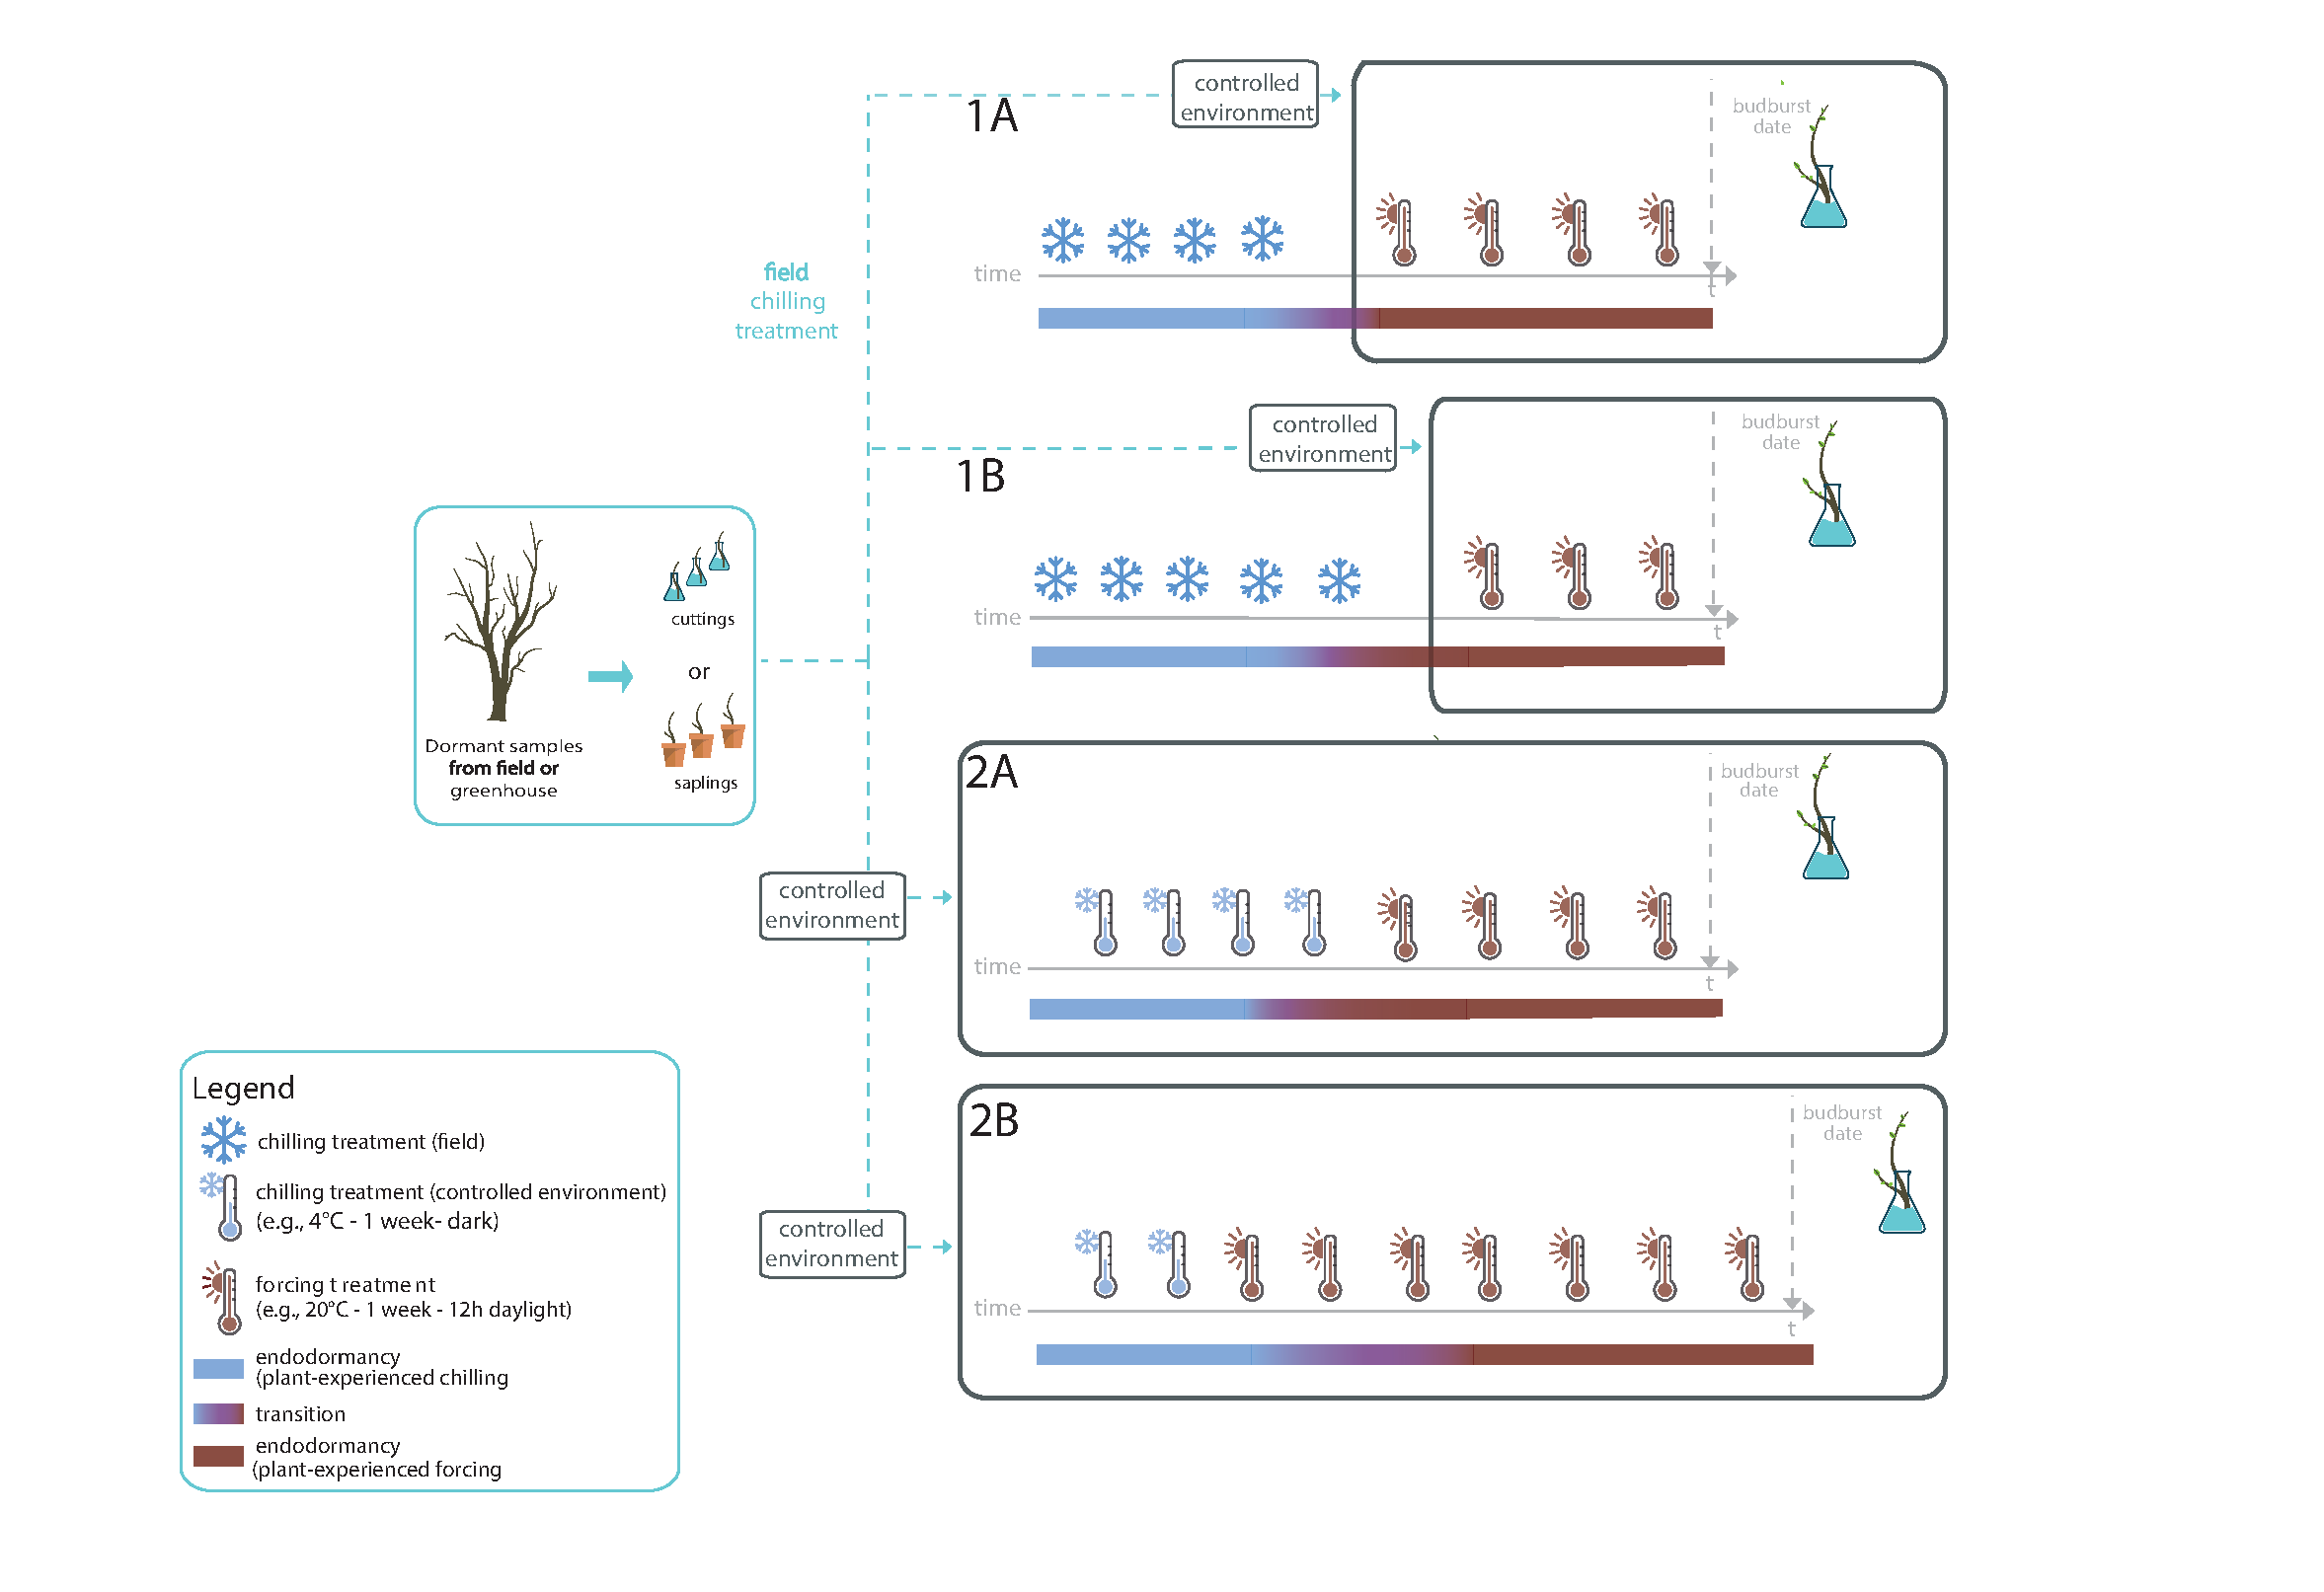
\includegraphics[width=1\textwidth]{figures/concept/Fig_bbconcept_dormant_V8.png}

\caption{\textbf{Short-term experiments on woody plant phenology manipulate photoperiod and temperature to estimate chilling, forcing, and photoperiod cues.} Chilling is manipulated by using natural chilling in the field (1A-B, in which plant material is collected after different numbers of days in the fall/winter) and/or experimentally (2A-B, in which plant material is placed in controlled environment chambers set to different chilling temperatures and/or durations). Chilling treatments are designed to break plant endodormancy, after which forcing treatments are imposed by moving plant material to warmer temperatures that allow budburst to occur. Ideally, this experimental transition aligns with the physiological shift from endo- to ecodormancy (e.g., 1A, though it could also occur with experimentally applied chilling). A challenge with these experiments is that species-specific chilling requirements are rarely known, so experimental treatments may not always align with what the plant experiences (\emph{i.e.}, physiological shifts in dormancy). Thus, in some cases, chilling treatments may bridge across what plants experience as both chilling and forcing (1B and 2A, where plants transition into ecodormancy before ``forcing'' treatments are applied), or chilling treatments may end before endodormancy is fully broken (2B). In the experiments synthesized here, photoperiod (not shown) is most often manipulated in forcing treatments. Across the 39 studies (found in 28 papers) included in our main model, we found treatments varied uniquely for each study, but some were more common than others, see Fig. \ref{fig:treatheatmaps}: chilling treatments across the averaged 71.4 days (range: 1-182 days) at an average temperature of 4.4 \degree C (range: 0-16 \degree C), forcing treatments averaged 15.7 \degree C (range: 5 to 32 \degree C).}
\label{fig:concept} 
\end{figure}

\begin{figure}[h!]
\centering
\noindent \includegraphics[width=0.75\textwidth]{..//..//analyses/bb_analysis/figures/muplotspcompexprampfputah_z.pdf}
\caption{\textbf{Estimated effects of chilling, forcing, and photoperiod on budburst timing across 65 species (modeled as 36 separate taxa, see the \emph{Models} section of \emph{Methods}) in 39 controlled environment experiments.} Using standardized units, which allow comparisons across cues, we show that most species (smaller symbols) are responsive to most cues, with chilling being the strongest cue when considering overall estimates across species (larger, dark blue circles). Overall estimates shown here were generally similar to other model formulations, including using data from 203 species (and 72 studies), and using different methods for calculating chilling (Fig. \ref{fig:lat}, \ref{fig:weinberger}; Tables \ref{tab:modsz}-\ref{tab:stage}). Lines represent 50\% uncertainty intervals (other intervals provided in Tables \ref{tab:modsz}-\ref{tab:stage})}.  
\label{fig:mu}
\end{figure}

\newpage

\begin{figure}[h!]
\centering
\noindent 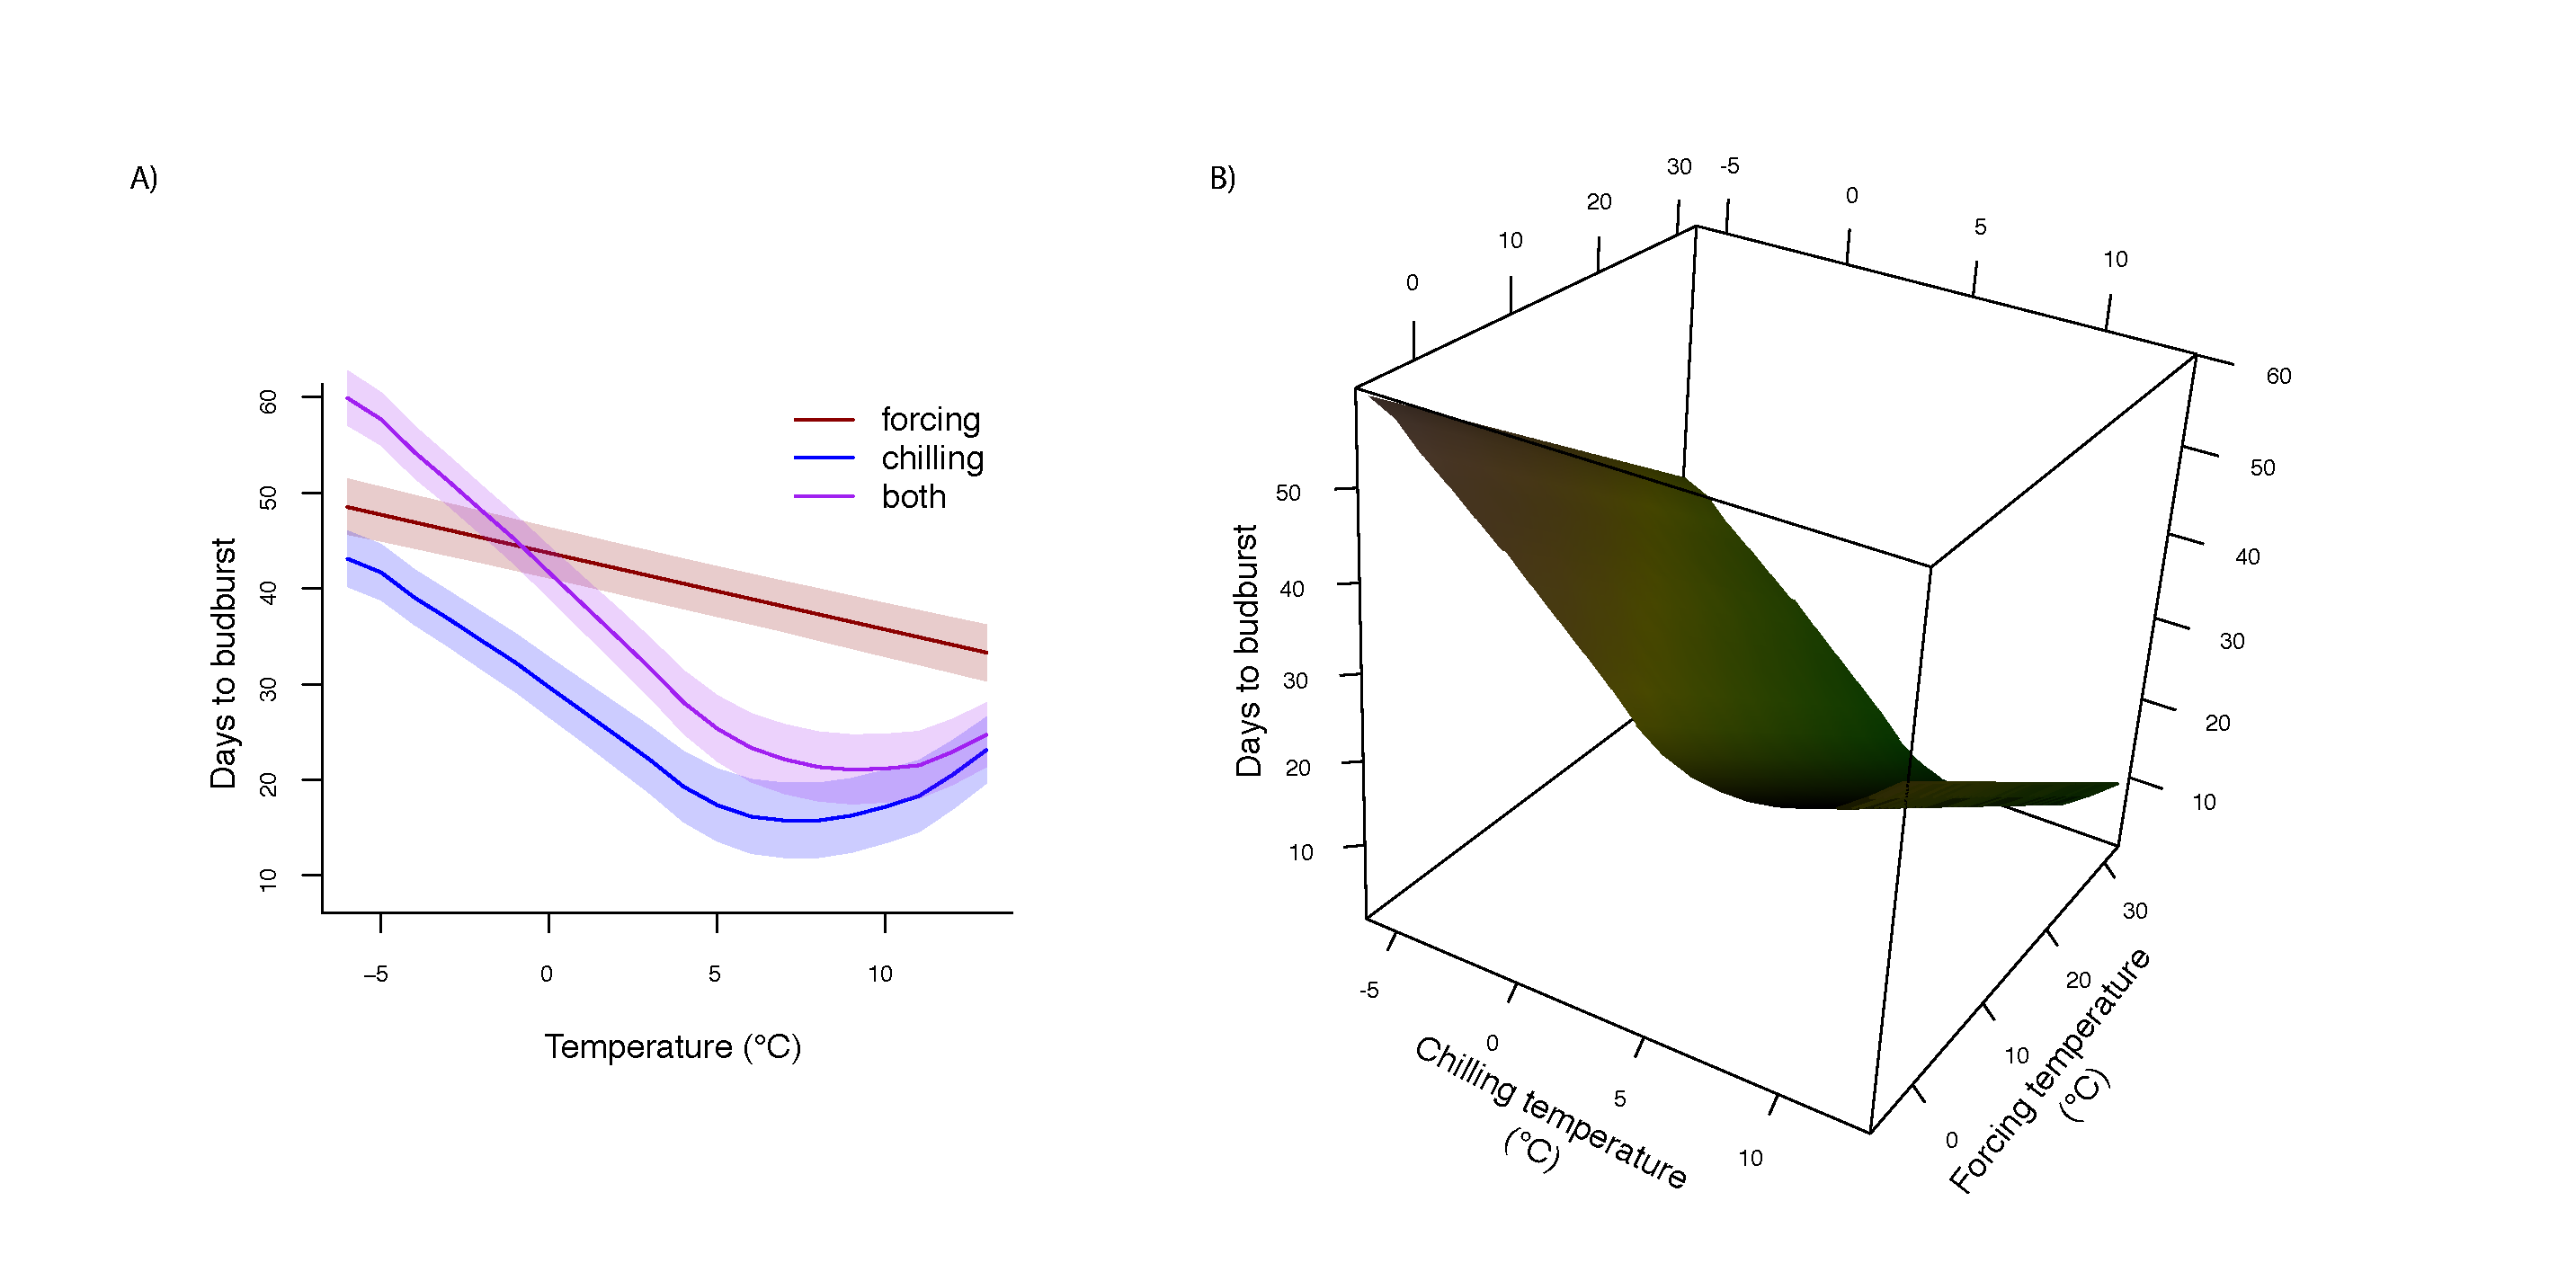
\includegraphics[width=1\textwidth]{..//..//analyses/bb_analysis/figures/bbmod_2d3dplot_utah_withPEP.pdf}
\caption{\textbf{Estimates of budburst across a range of forcing temperatures and estimated chilling} (converted to a representative mean temperature, see \emph{Estimating chilling} in Methods) based on overall estimates of chilling and forcing effects from a meta-analysis of short-term experiments using controlled temperature and/or photoperiod conditions (Fig. \ref{fig:mu}). Note that days to budburst is relative to experimental methods and thus not comparable to day of year in the field, shading (in A) represents 50\% uncertainty intervals. Panel A shows the effect of chilling temperature on budburst, with forcing kept at the mean level across all experiments (16\degree C); the effect of forcing temperature with chilling kept at the mean level across all experiments (1324 chilling units), and the effect of varying both chilling and forcing temperatures simultaneously. Panel B shows all possible combinations of chilling and forcing across the experimental conditions.
Maximum advances in budburst occur at intermediate chilling temperatures (\emph{e.g.}, here at mean winter temperatures of 6-7\degree C) and the highest forcing (here at 32\degree C). We set photoperiod to eight hours, which is the most common photoperiod treatment in our meta-analysis.}
\label{fig:3dfieldchillutah}
\end{figure}


\begin{figure}[h!]
\centering
\noindent 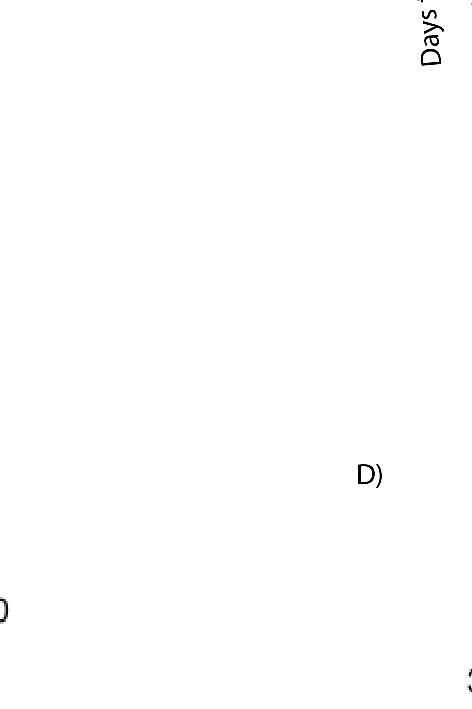
\includegraphics[width=0.75\textwidth]{..//..//analyses/bb_analysis/figures/forecasting/tempforecastbothspp_1_7_degwarm3D_utah.png}
\caption{\textbf{Implications of warming on budburst timing varies across species and sites}, depending strongly on pre-warming climate conditions related to chilling for each site. Here we show species-level estimates from our model based on a meta-analysis of experiments (Fig. \ref{fig:mu}) for two common species \emph{Betula pendula} (A, B) and \emph{Fagus sylvatica} (C, D), based on climate data from two sites in Central Europe (these two sites chosen to highlight the diversity of possible budburst responses to warming, see Fig. \ref{fig:foremap} for general trends across many sites in the same region). In some sites, warming increases total chilling estimates (A, C) leading to greater advances in budburst (compared to forcing alone), whereas warming decreases total chilling estimates in other sites (B, D), leading to smaller advances and, eventually, delays with substantial warming. See Fig. \ref{fig:betfag2d} in the Supplemental Materials for a simplified two-dimensional version.}
\label{fig:betfag3d}
\end{figure}

%%%%%%%%%%%%%%%%%%%%%%%%%%%%%%%%%%%%%%%%
\end{document}
%%%%%%%%%%%%%%%%%%%%%%%%%%%%%%%%%%%%%%%%
